% options:
% thesis=B bachelor's thesis
% thesis=M master's thesis
% czech thesis in Czech language
% slovak thesis in Slovak language
% english thesis in English language
% hidelinks remove colour boxes around hyperlinks

\documentclass[thesis=B,czech]{FITthesis}[2012/06/26]

\usepackage[utf8]{inputenc} % LaTeX source encoded as UTF-8

\usepackage{graphicx} %graphics files inclusion
% \usepackage{amsmath} %advanced maths
% \usepackage{amssymb} %additional math symbols

\usepackage{dirtree} %directory tree visualisation
\usepackage{float}

\usepackage{listings}

% % list of acronyms
% \usepackage[acronym,nonumberlist,toc,numberedsection=autolabel]{glossaries}
% \iflanguage{czech}{\renewcommand*{\acronymname}{Seznam pou{\v z}it{\' y}ch zkratek}}{}
% \makeglossaries

\newcommand{\tg}{\mathop{\mathrm{tg}}} %cesky tangens
\newcommand{\cotg}{\mathop{\mathrm{cotg}}} %cesky cotangens

% % % % % % % % % % % % % % % % % % % % % % % % % % % % % % 
% ODTUD DAL VSE ZMENTE
% % % % % % % % % % % % % % % % % % % % % % % % % % % % % % 


\department{Katedra softwarového inženýrství}
\title{Systém pro správu elektronických verzí literárních děl}
\authorGN{Martin} %(křestní) jméno (jména) autora
\authorFN{Melichar} %příjmení autora
\authorWithDegrees{Martin Melichar} %jméno autora včetně současných akademických titulů
\supervisor{Ing. Karel Klouda, Ph.D.}
\acknowledgements{V prvé řadě bych rád poděkoval panu Ing. Karlu Kloudovi, Ph.D. za pomoc, trpělivost a odborné rady v průbehu psaní této bakalářské práce a za možnost podílet se na reálném projektu, který se bude pravděpodobně v praxi používat. Dále bych chtěl poděkovat své přítelkyni a rodině za trpělivost a podporu v průběhu studia na ČVUT. }
\abstractCS{
Cílem této bakalářské práce je ulehčit převod literárních děl do elektronické podoby. Vytvořené řešení dovoluje upravovat, mazat nebo přidávat dílčí součásti knihy např. autora díla a také spravovat přidružené přílohy k jednotlivým dílům. Systém je napsán v PHP pomocí microframeworku Slim. Hlavním výsledkem je zrychlení vytváření a snadné upravování elektronických verzí literárních děl.

}
\abstractEN{The aim of this thesis is to facilitate the conversion of literary works into electronic form.}
\placeForDeclarationOfAuthenticity{V~Praze}
\declarationOfAuthenticityOption{4} %volba Prohlášení (číslo 1-6)
\keywordsCS{webová aplikace, redakční systém, návrh a implementace, správa eletronických literárních děl, Slim, PHP}
\keywordsEN{web application, management system, design and implementation, digitalized literary works, Slim, PHP}

\setcounter{tocdepth}{2}
\setcounter{secnumdepth}{2}

\begin{document}

% \newacronym{CVUT}{{\v C}VUT}{{\v C}esk{\' e} vysok{\' e} u{\v c}en{\' i} technick{\' e} v Praze}
% \newacronym{FIT}{FIT}{Fakulta informa{\v c}n{\' i}ch technologi{\' i}}

\begin{introduction}
	%sem napište úvod Vaší práce

    Elektronická literární díla stále rozšiřují pole své působnosti, ať mluvíme o nakupování nebo zobrazování knih na počítači či o jejich snadném čtení v e-čtečkách. V Austrálii se rozdíl prodeje elektronických knížek v roce 2008 oproti roku 2009 rapidně zvýšil, a to o více než 100 \%. Ve Spojených státech amerických se v lednu roku 2012 zvýšil prodej e-knih pro dospělé o 49,4 \% a e-knih pro děti a mládež o 475,1 \%, než tomu bylo v lednu 2011 \cite{info}. Zde vidíme prudký nárůst prodeje e-knih, z toho můžeme usoudit, že rapidně roste oblíbenost elektronických děl. Zobrazení a následné čtení e-knih na našich elektronických zařízení je nejenom snazší, ale i pohodlnější oproti zapůjčování či koupi papírových knih.

	Výsledek této práce je přednostně určen pro zaměstnance Ústavu české literatury Akademie věd České republiky (UČL AV). Pracovníci ústavu získávají, ať formou darů či koupí, postupně více literárních děl. Tato díla následně naskenují a převedou do elektronické podoby. Nicméně často to bývají historická díla, a proto se stává, že naskenovaný výsledek přesně neodpovídá tištěné podobě knihy. Proto je nezbytné, aby pracovníci ústavu ručně opravovali chyby a měli možnost doplňovat chybějící části v elektronické podobě díla. Zde přichází na řadu aplikace, která bude umožňovat rychlejší a efektivnější úpravu nově vzniklého díla.

	Na základě poznámek a připomínek zaměstnanců bude tato aplikace efektivní a upravená na míru. Toto téma jsem si zvolil, protože je velmi aktuální a výsledek by mohl výrazně ulehčit práci při vytváření literárních elektronických děl.

    \section{Cíl práce}
    
        Prvním cílem je rešerše existujících aplikací pro tvorbu a správu literárních děl a dále porovnání a výběr nejvhodnějšího frameworku pro tvorbu aplikace. S tím úzce souvisí výběr samotného jazyka pro implementaci. Poté přijde na řadu  porovnání a volba nejvhodnějšího textového formátu pro e-knihy. Dalším krokem je shromáždění poznámek a připomínek od pracovníků pro vytvoření aplikace na míru.
    
        Cílem praktické části práce je navrhnout a implementovat redakční systém pro správu a snadné vytváření elektronických verzí literárních děl, otestovat systém na reálných datech a uživatelích a řádně jej zdokumentovat. Systém bude umožňovat správu nejen samotných dokumentů, ale i souborů k nim přidruženým, zejména fotografií a obrázků. Ve výsledné aplikaci bude implementován jednoduchý filtr a snadné vyhledávání v seznamu sbírek. Aplikace bude umožňovat autentifikaci a bude zároveň poskytovat správu uživatelů a jejich rolí. V aplikaci bude administrátorovi umožněna registrace nového uživatele, který si následně upraví heslo podle své potřeby.
        
    \section{Úvod do problematiky}

        V současnosti mají pracovníci UČL AV okolo 1700 literárních děl uložených v databázi ve formátu XML. Díla jsou rozdělena do dvou částí, jak je vidět na příkladu Vytržené listy \ref{fig:xml}. První část je identifikována tagem hlavička a druhá tagem text. Hlavička obsahuje metadata jako je titul díla nebo rok vydání a ve druhé části je samotný text rozčleněn například do tagů sbírka a báseň.
        
\end{introduction}

\chapter{Analýza}

    \section{Existující řešení}
        Před návrhem a implementací aplikace bylo potřeba řádně prozkoumat existující řešení problému, technologií k tvorbě a elektronické formáty, které se užívají pro uchování elektronických děl. Vzhledem k roztoucí poptávce po elektronických děl na úkor papírových se podle očekávání objevilo spoustu aplikací pro editaci těchto děl.\\
        Podle serveru \cite{tei-wiki} pět editorů
        \begin{itemize}
            \item Emeditor
            \item Editix
            \item EditPad Pro
            \item Essential XML Editor 
            \item Exchanger XML Editor
        \end{itemize}

        \subsection{Emeditor}
            Emeditor\footnote{domovská stránka: \url{https://www.emeditor.com/}} patří mezi nejlepší XML editory. Tento software je hlavním produktem americké firmy Emurasoft, Inc. sídlící v Redmondu ve Washingtonu. Firma se nadále stará o podporu i vývoj. Nicméně autorem editoru je Yutaka Emura. Samotná aplikace již vyhrála 24 mezinárodních cen v kategoriích nejlepší webový nástroj nebo nejlepší aplikace roku 2008. 
            
            \subsubsection{výhody}
                \begin{itemize}
                    \item poslední release v17.5.0 vyšla 27.\,února\,2018
                    \item podpora velkých souborů
                    \item použití více jader při větší zátěži
                    \item kódování UTF-8
                    \item konfigurovatelná kontrola pravopisu
                \end{itemize}
                
            \subsubsection{nevýhody}
                \begin{itemize}
                    \item aplikace je placená, ale nabízí trial verzi na 30 dní
                    \item existuje free verze, nicméně v ní chybí zásadní funkce
                    \item editor je pouze pro Windows
                    \item chybí přehledný průvodce základních funkcí po prvním spuštění
                \end{itemize}
                
        \subsection{Editix} 
            Editix\footnote{domovská stránka: \url{http://www.editix.com/index.html/}} je produktem francouzské společnosti JAPISoft SARL. Editor vytvořil Alexandre Brillant. Systém je velice přehledný a intuitivní. Na trhu systém je od roku 2004 a nejnovější verze je EditiX XML Editor 2017 v15. Zákaznící, kteří využívají tento software jsou převážně vzdělávací instituty od University of Oxford po University of Arizona.
            
            \subsubsection{výhody}
                \begin{itemize}
                    \item přehledný program
                    \item aplikace je pro platformy Windows, Linux, MacOS	
                    \item existuje EditiX Community Edition, která je zadarmo
                    \item mnoho užitečných funkcí např. Find and Replace
                    \item obsahuje inteligentní našeptávač, který pomáhá uživatelům
                \end{itemize}
                
            \subsubsection{nevýhody}
                \begin{itemize}
                    \item verze pro je placená, ale nabízí trial verzi na 30 dní
                    \item existuje lite verze, které chybí spoustu funkcí
                    \item zaplacení licence se vztahuje pouze na jednoho uživatele
                    \item první update je zdarma, další se musí zaplatit
                \end{itemize}
                
        \subsection{EditPad Pro}
            EditPad Pro\footnote{domovská stránka: \url{http://www.editpadpro.com/}} je výhradně textový editor, který lze použít například pro HTML, Javascript nebo XML. Software podporuje změnu jazyka napřiklad do francouzštiny, němčiny, polštiny nebo švédštiny. Projeck Just Great Software, pod kterým byla vyvynuta tato aplikace vznikl v roce 1996. Autorem projektu je Jan Goyvaerts, který je zároveň hlavním ředitelem vývojářu projektu.

            \subsubsection{výhody}
                \begin{itemize}
                    \item program je obecný textový editor
                    \item obarvená syntaxe
                    \item dobře pracuje s velkými soubory
                    \item podpora UTF-8
                    \item existuje EditPad Lite verze, která je zdarma
                \end{itemize}
                
            \subsubsection{nevýhody}
                \begin{itemize}
                    \item nemá explicitní podporu pro XML
                    \item aplikace je pouze pro Windows
                    \item chybí vyhledávání v souborech
                    \item verze Pro je placená, ale existuje verze Lite
                \end{itemize}
                
        \subsection{Essential XML Editor}
            Essential XML Editor\footnote{domovská stránka: \url{http://www.philo.de/xmledit/}} je jednoduchý XML editor. Jeho klíčovou vlastnostní je vestavěný XML validátor. Vývojáři dříve pojmenovali program Open XML Editor, ale po zavedení poplatku za některé funkce projekt přejmenovali. Autorem je Dieter Köhler. 
            
            \subsubsection{výhody}
                \begin{itemize}
                    \item program pracuje jako textový editor
                    \item možnost rychle zjistit zda je soubor validní
                    \item trial verze není časově omezená
                    \item vstupní soubor může být v různém kódování
                    \item klávesová zkratka pro každý příkaz
                \end{itemize}
                
            \subsubsection{nevýhody}
                \begin{itemize}
                    \item výstupní soubor pouze v UTF-8 kódování
                    \item aplikace je pouze pro Windows
                    \item pro zpřístupnění některých funkcí nutnost zakoupit klíč
                    \item poměrně zastaralý desing aplikace
                \end{itemize}

        \subsection{Exchanger XML Editor}
            Exchanger XML Editor\footnote{domovská stránka: \url{http://www.exchangerxml.com/editor/}} je určen pro snadnou editaci, prohlížení, správu a konverzi XML souborů. Exchanger pomáhá svojí širokou nabídkou funkcí XML autorům a vývojářům.  Software je prouktem firmy Cladonia, která se zaměřuje na vývoj XML aplikací. 
            
            \subsubsection{výhody}
                \begin{itemize}
                    \item nabízí full verzi na 30 dní
                    \item aplikace je dotupná na všech platformách
                    \item možnost zobrazení základního náhledu
                    \item poskytuje podporu pro TEI formou stáhnutí balíčku
                    \item automatická kotrola, jestli je soubor validní
                \end{itemize}
                
            \subsubsection{nevýhody}
                \begin{itemize}
                    \item při instalaci nutnost najít cestu k JRE manuálně
                    \item zastaralý software
                    \item časově neomezenou verzi je nutno zakoupit
                    \item poslední update proběhl v roce 2010
                \end{itemize}
                
    \section{Stávající aplikace}
        V současné době mají pracovníci UČL AV k dispozici aplikaci, která byla vyvinuta již v roce 2006. Serverová část (back-end) aplikace běží v node.
        
        \subsection{Aktuální stav}
        Tato aplikace je na první pohled podstatně zastaralá, a to jak v uživatelském rozhraní, tak i ve funkční části programu. To je způsobeno zastavením veškerého vývoje a podpory již před několika lety.

        \subsection{Nedostatky}
            Uživatelé pracující s aplikací si často stěžují například na rychlost běhu nebo na nemožnost přidávat chybějící části díla.
            
    \section{Technologie}
        Mezi první otázky projektu patřilo, v jaké technologii se bude psát. Po domluvě s pracovníky UČL AV jsem měl vytvořit webovou aplikaci, která je technologicky podobná té stávající. Aplikace měla mít přívětivé uživatelské rozhraní pro snadnou a rychlou správu elektronických děl neměla obsahovat zásadná chyby jako dřívější aplikace. 
        
        Další duležitou otázkou bylo, ve kterém elektronickém formátu se budou díla tvořit a uchovávat. Existuje celá řada formátů, proto bylo pro budoucí možné rozšíření duležité domluvit se s pracovníky na správném formátu.
        
        \subsection{Jazyk}
            U jednoduchých webových aplikací postačí, když klientská strana pošle požadavek na serverovou část, ta jej vyhodnotí a pošle odpověď zpět. Pro implementaci tohoto případu se nejčastěji používá architektura client/server \cite{languages}. 
            
            Jedna z výhod pro tuto architekturu je, že klientská strana programu je oddělena od serverové části. Výpočty jsou prováděny na straně serveru, proto nejsou požadovány vysoké nároky na výpočetní techniku počítače, na kterém běží klientská část. Probíhá zde věrší ochrana duležitých dat, protože všechny jsou uchovávány na serverové části.
            
            Nevýhodou může být vysoká cena zařízení pro provoz nebo pro správu serveru je potřeba systémového administrátora.\\
            Srovnání jazyků pro webové aplikace:
            
            \begin{itemize}
                \item PHP – jeden z nejrozšířenějsích jazyků, který podporoje většina poskytovatelů webhostingu. Tento jazyk je široce využíván mezi uživateli a obsahuje spostu standardních knihovních funkcí. Hodí se pro malé nebo středně velké projekty.
                \item Ruby – navzdory tomu, že Ruby je mladý jazyk, těší se velké oblíbenosti mezi webovými vývojáři. Nejznámější framework Ruby on Rails umožňuje rychle vytvářet vzorové nebo malé projekty, avšak neprochází všemi časovými testy, a proto velmi pravděpodobně obsahuje zásadní chyby. Pro nové uživatele je z důvodu daných pravidel Ruby on Rails složitý na implementaci nezbytných funckí.
                \item Perl – momentálně vývoj jazyku probíhá velice pomalu, jeho použití ve větších webových projektech je spíše vzácností.
                \item Python – díky nástupu velkých frameworků - například Django, je možné použit Python ve velkých webových projektech. Syntaxe kódu je podobná Ruby, ale hlavní rozdíl činí ideologie psaní kódu. Nicméně narozdíl od Ruby se Python rozvíjí rychleji.
                \item C\# ASP.NET – pro správné fungování jazyka je třeba zařídit ISS server, který je nezbytný pro mnoho komerčních projektů od firmy Microsoft. Jiným řešením může být použítí serveru Mono, který ale není stabilní a může obsahovat mnoho chyb.
                \item JAVA – tento široce využívaný jazyk lze aplikovat na velké či korporační projekty. Je poměrně rychlý a obsahuje spoustu již vyřešených složitých problémů, které nemusí uživatel znovu řešit. Pro začátek je vyžadováno poměrné velké množství znalostí, aby fungovala základní kostra programu, což se považuje za významnou nevýhodu.
            \end{itemize}
            
            Pro tento projekt postačí menší a jednoduší aplikace, kterou zaměstnanci UČL AV snadno nahrají na jejich servery, a proto byl na základě této analýzy vybrán jazyk PHP.
            
        \subsection{Databáze}
            Srovnání několika open-source databázových řešení podle \cite{database}\\
            \begin{itemize}
                \item CUBRID\footnote{domovská stránka: \url{https://www.cubrid.org/}} – byl navržen a optimalizován pro webové aplikace. Hodí se pro práci s velkými daty, nebo při nutnosti použití více dotazů najednou. Výhodou je možnost online zálohy a grafické rozhraní pro jazyky PHP, Python, Perl a Ruby. N druhou stranu manuál existuje pouze v angličtině nebo korejštině. Spoustu příspěvku na forum jsou řadu let stará.
                \item Firebird\footnote{domovská stránka: \url{http://www.firebirdsql.org/en/start/}} – je prvním zástupcem relační databáze. Systém fungujícá již od roku 1981, který lze použít na Linux, Windows a další Unixové platformy. Firebird má obsáhlou komunitu, uživatel může využít spoustu vývojářských nástrojů a obsahuje autentizaci skrz Windows účet. Naopak chybí dočasné tabulky a integrace mezi ostatnímy databázovými systémy.
                \item MariaDB\footnote{domovská stránka: \url{https://mariadb.org/}} – byla vytvořena původnímy vývojáři MySQL. MariaDB využívají dnes největší společnosti jako jsou Google nebo Facebook. Proto je ochrana dat na špičkové úrovni. Díky působení na trhu již přes 20 let patří mezi nejvýkonější systémy. Jako nevýhoda se dá počítat chybějící plugin password complexity.
                \item MongoDB\footnote{domovská stránka: \url{https://www.mongodb.com/}} – byl vytvořen v roce 2007 jako řešení pro větší projekty. Díky svým sponzorům a podporovatelům si uchovává myšlenku být jednoduchý a přirozený. Dokáže zpracovat poměrně rychle velké množství dat a po hlavní závadě nastupuje rychlé obnovení.
                \item MySQL\footnote{domovská stránka: \url{https://www.mysql.com/}} – funguje již od roku 1995. Dnes je využívána jako standardní databáze pro menší i větší projekty. Běží na všech známých operačních systémech a lze použit, ikdyž není funkční síť. Velkou výhodou nabízí oddělený server od vývojového prostředí. Trochu uvadá komunita a nové aktualizace přichází čám dál tím později. 
                \item PostgreSQL\footnote{domovská stránka: \url{https://www.postgresql.org/}} – má za sebou 15 let aktivního vývoje a patří mezi systémy, které běží na všech hlavních operačních systémech. S použitím PostgreSQL může uživatel vytvořit vlastní metody nebo nestandardní datové typy. Mnoho věstavěných procedur lze spouštět skrze mnoho programovacích jazyků, jako je Java, Perl, Python nebo C/C++. Nastává problém při vysokém počtu transakcí a vývoj je řízen pouze komunitou.
                \item SQLite\footnote{domovská stránka: \url{https://www.sqlite.org/index.html}} – se sama považuje za nejrozvinutější datavázi na světě. Vývoj začal v roce 2000 a použivali jej významné firmy jako je Facebook, Apple nebo Microsoft. Před každém release musí být kód pečlivě zkontrolován, aby se předešlo případným chybám. Poté vývojáři zveřejní přesný výčet změn. K dispozivi je kvalitní podpora a knihovna, která pracuje rychle na úkor velikosti paměti. SQLite se nedoporučuje pro obsáhlé webové aplikace a velké množství dat.
        \end{itemize}
        
        Na základě zjištění a protože tento projekt bude patřit spíše k těm menším, byla vybrána databáze SQLite.
        
        \subsection{Elektronický formát}
            \uv{\textit{Mezi formáty, v nichž můžeme číst elektronickou literaturu, jsou jednak ty, které byly pro tento účel přímo vytvořené, ale také ty, v nichž se e-knihy publikovaly prostě proto, že nebylo mnoho jiných alternativ. Toto se týká zejména stavu v 90. letech, kdy vznikaly kopie (převážně papírových) knih převedené do formátů jako jsou TXT, HTML či RTF.}}\cite{electronic-format}
            
            Elektronickému formátu je třeba věnovat zvláštní pozornost, protože se do buducna počítá s rozšířením aplikace o část, která se bude věnovat zobrazením těchto děl.
            
            Seznam vybraných formátů pro e-knihy uvedené v \cite{electronic-format}
            
            \begin{itemize}
                \item Archos Diffusion – je formát vytvořen franouzskou firmou  ArchosDiffusion. Koncovka názvů souborů je .aeh. Formát byl vytvořen pro uchovávání literatury v elektronické podobě a patří do skupiny formátů založených na XML. Otevírat soubory lze v programu Archos Player nebo ve volně dostupné aplikaci Visual Vision EbooksReader. Postupem času uvadá zájem o tento formát.
                \item AZW – formát vyvinuli vývojáři Amazonu a používá koncovku .azw. Tento formát byl v zhotoven pro uchování elektronických děl v internetovém knihkupectví společnosti Amazon. Knihy lze číst ve všech dostupných verzích čteček Kindle i v prostředí softwarových čteček. Díky oblíbenosti čteček Kindle patří AZW mezi nejrozšířenějších formáty na světě. Velkou nevýhodou je jeho uzavřenost, protože knihy ve formátu AZW prakticky nelze číst v jiných čtečkách než jsou Kindle.
                \item EPUB – je součástí nejpopulárnějších formátu na světe i v České republice. Vytvořilo jej sdružení International Digital Publishing Forum a je založený na XML. Knihy ve formátu EPUB lze číst na většině čtecích zařízeních s výjimkou čteček Kindle, nicméně existuje možnost převodu formátu EPUB do jiného, který dokáží číst i čtečky Kindle. Tento otevřený formát podporuje Digital rights management (DRM) ochranu a proto si získal oblibu i u nakladatelů.
                \item Hypertext Markup Language – se primárně používá pro tvorbu webocýh stránek. V 90. letech, kdy se začaly poprvé vytvářet elektroncké podoby knih, nebyl ještě vyvinut žádný formát pro jejich zobrazení, a proto se z nutnosti používal také HTML. Převod probíhal pomocí naskenování díla a přes Optical Character Recognition (OCR) aplikaci samotný převod do formátu HTML. Ke čtení postačil webový prohlížeč. Nicméně s nástupem formátů navržených pro elektronické knihy se přestal HTML používat.
                \item Portable Document Format – vyvinutý společností Adobe v roce 1993 byl primárně určen pro uchování souborů pro tisk. Patří mezi formáty, které nebyly vytvořeny pro elektronickou literaturu, ale narozdíl od ostatních, se tak používá dodnes. Velkou předností je nezávislot na platformě, protože s PDF lze pracovat téměř na všech operačních systémech. 
                \item Plain text – patří mezí formáty, které nebyly určeny pro uchovávání e-knih. V 90. letech se používal pro zobrazení elektronické literatury, protože nebylo tolik jiných možností. Díky malé datové velikosti souborů a možnosti čtení souborů neomezeně na platformě se stále používá. TXT nedovoluje formátování a nepodporuje vložení obrázků, videí či zvukových stop.
                \item Text Encoding Initiative – byl vytvořen TEI konsorciem primárně pro elektronickou literaturu. Formá je využíván ve výukových projektech i knihovnách po celém světě. Řadí se do skupiny formátů, které jsou založeny na XML. TEI se označuje jako nastavitelný, protože uživatel může podle své vůle přidat, předefinovat nebo přejmenovat tagy a jejich atributy. Formát se dá použít pro různé druhy textů.
            \end{itemize}
            
            Drtivá většina děl dostupná pracovníkům UČL AV je právě ve formátu XML. Avšak tento formát není primárně určen pro uchovávání elektronických verzí literárních děl, proto byl pro mou práci vybrán textový formát TEI.
    \section{Software}
        \subsection{Microframework vs framework}
            Následující analýzu jsem provedl podle \cite{microframework-vs-framework}
            
            Framework poskytuje skoro vše, co programátor potřebuje, od obsluhy webových požadavků po řízení databáze. Obsahuje i komponenty, které vývojář nemusí nikdy použít, nicméně z hlediska rozšířitelnosti jsou výhodné.
            
            Microframework je označením pro framework, který obsahuje pouze potřebné komponenty k vývoji webové aplikace. Microframeworky bývají přizpůsobeny menším aplikacím nebo aplikacím s konkrétním účelem. Pro rozšíření funkčnosti je potřeba přidat dané komponenty.
            
            Reálně je microframework sbírka nutně potřebných komponent k webové aplikaci. Obsluha microframeworku dostane HTTP požadavek, který zpracuje daný kontroler a pošle odpověď zpět. Některé microframeworky obsahují další nástroje pro manipulaci s HTTP požadavky. Mnoho vývojářů používá raději velké frameworky, jako jsou Laravel nebo Symfony. Tyto frameworky disponují spoustou již vyřešených problému a mají velikou programátorskou základnu. Nicméně potřebují více času pro pochopení a porozumění prostředí. 
            
            Jsou projekty, u kterých se vyplatí použít velké frameworky, ale v případě projektů, kde není potřeba tolik funkcí, je vhodné použít microframework. Tento projekt se charakterizuje spíše menší náročností a nebude obsahovat složité požadavky. Aplikace nebude mít mnoho stránek a proto ideláním řešením bude microframework.
            
            5 nejlepších microframeworků podle \cite{microframeworks}
            
            \begin{itemize}
                \item Slim\footnote{domovská stránka: \url{https://www.slimframework.com/}} – je považován za jeden z nejlepších PHP microframeworků. Umožnuje snadno vytvořit komplexní webovou aplikaci. Díky nastavitelné a modulární architektuře poskytuje vývojářům přesně to, co potřebují. Slim dovoluje vkládat závislosti, proto jej lze použít společně s externími nástroji.
                \item Silex\footnote{domovská stránka: \url{https://silex.symfony.com/}} – byl vyvinut z frameworku Symfony, aby byl co nejmenší a zároveň poskytoval základní funkčnost. Nakonec vznikly dvě verze. Fat verze má v sobě komponenty ze Symfony, Twig, šablonovací systém a jiné. Druhá slim verze obsahuje základní systém routování a několik procedur. 
                \item Wave\footnote{domovská stránka: \url{https://www.waveframework.com/}} – používá architekturu model-view-control. Neobsahuje doplňkové knihovny a klade důraz na rychlost a optimalizaci. Wave podporuje jQuery JavaScript framework.
                \item Limonade\footnote{domovská stránka: \url{https://limonade-php.github.io/}} – se zaměřuje obdobně jako Wave na jednoduchost. V Lumenu je velmi rychlé a snadné napsat základní aplikaci. Nicméně je až extrémně malý a nelze jej rozšířit o složitější funkčnost. Spoléhá pouze na globální funkce.
                \item Lumen\footnote{domovská stránka: \url{https://lumen.laravel.com/}} – je microframework odvozený ze světoznámého PHP frameworku Laravel. Pokud si programátor není jistý velikostí svého projektu, je výhodné použít Lumen, protože stačí veškerý kód z Lumenu převést do Laravelu a vše bude fungovat jak má.
            \end{itemize}
        
        Po prostudování a podrobné analýze současně dostupných microframeworků byl vybrán Slim. Zároveň chci použít šablonovací systém TWIG, který Slim podporuje.
        
    \section{Grafické nástroje}
        podle jakých nástrojů jsem dělal grafické návrhy
    

\chapter{Návrh aplikace}

    \section{Wireframy}
        co to je, proč jsem je udělal
        \subsection{Login}
            
        \subsection{Hlavní stránka}
        
        \subsection{Metadata}
        
        \subsection{Přílohy}
        
        \subsection{Autoři a vydavatelé}

    \section{Databázové schéma}
        jaké jsem vybral
    \section{Zabezpečení}
        jak je zabezpečené heslo uživatele

    
\chapter{Implementace}
    Při vytváření kódu bylo nutné dodržovat domluvené návrhy. Kód musel být přehledný pro případné rozšířění aplikace jiným vývojářem. Díky vybranému softwaru a jeho přívětivé příručce byla poměrně rychle vytvořena aplikace v základní podobě. Slim má obrovskou komunitu uživatelů, což je velice nápomocné při hledání řešení problému. 

    \section{Import}
        Ještě před implementací se musely do databáze aplikace zpracovat sbírky z UČL AV. Podle očekávání byla data dodána ve formátu XML. Import nedoprovázely žádné komplikace zejména díky snadné ovladatelnosti a standardním knihovnám scriptovacího jazyka Python\footnote{domovská stránka: \url{https://www.python.org//}}. Současně s importem sbírek proběhlo zpracování příloh k nim přidružených.
        
        \subsection{Stávající sbírka děl}
            Stávající díla mají pracovníci z UČL AV v databázi. Část z této sbírky děl je ústavem již zpracována, na zbylé části se stále pracuje. Dříve byla tato díla upravována pomocí kancelářského balíčku Microsoft Word\footnote{domovská stránka: \url{https://products.office.com/cs-cz/word}}. Word je skvělý nástroj pro editaci jednotlivých souborů, nicméně nedovoluje spravovat soubory jako celek. V současné době pracovníci UČL AV čekají na novou aplikaci, protože jim chybí vhodný nástroj k úpravě děl.
            
            Import literárních děl proběhl otevřením každého souboru a zpracováním skriptem. Skript získal informace o dílu, vytvořil nové nebo navázal na již existující autory či vydavatele a vytvořil záznamy v tabulkách. Pro práci s XML byla použita standardní knihovna ElementTree\footnote{domovská stránka: \url{https://docs.python.org/2/}}. Python má stejnojmenou knihovnu pro práci s databází sqlite.
            
            V~ElementTree se na začátku zavolá funkce getroot. Tato funkce inicializuje proměnnou, ve které je obsah souboru a  dá se v ní snadno přistupovat k jednotlivým tagům. Tag hlavicka indikuje údaje o dílu a obsah díla patří pod tag text. Funkce find slouží k nalezení a vrácení tagu podle jeho názvu.
            
            Fulltextové vyhledávání v aplikaci vyžaduje text bez tagů. K tomu slouží funkce itertext, která ignoruje tagy a vrátí celý text. Naopak funkce pro získání obsahu včetně tagů není v ElementTree vestavěna. Nicméně potřebný text lze dostat spojením jiných funkcí. Obsah této funkce byl inpirován \cite{fn01}. 
            
            Některá díla mají více autorů. V takovém případě všechna jména zapsána v tagu author. Tato jména jsou ohraničena množinovými závorkami a oddělena středníkem. Mnoho autorů si v průběhu své tvorby vymyslelo pseudonym. Pseudonym autora je indikován znakem \uv{=}. Vlevo od znaku je pseudonym a vpravo je pravé jméno autora. Funkce doAuthors vrací id autora nebo pole id autorů v závislosti na vstupním parametru authors. Tento parametr je typu string a pokud začíná znakem \uv{\{}, má dílo více autorů. Pro tento případ funguje funkce jako rekurze. Druhým parametrem funkce je indikátor rekurze (recursion).
            
            Pro ilustraci je uveden začátek funkce zpracování autorů díla.
             \begin{minted}[frame=single, autogobble=true, label=doAuthors]{python}
def doAuthors(authors, recursion):
    #there is no author
    if (authors == 'neznamy'):
        return -1
    #there are more authors
    if (authors[0] == '{'):
        authors = authors.replace('{', '')
        authors = authors.replace('}', '')
        authArr = authors.split(';')
        authArr[0] = ' ' + authArr[0]
        out = []
        for authorName in authArr:
            out.append(doAuthors(authorName, 1))
        return out
    #there is only author 
    elif (authors.find('=') == -1):
        authors = authors.replace('(', '')
        authors = authors.replace(')', '')
        lastName, sep, name = authors.partition(',')
        name = name[1:]
        if (recursion == 1):
            lastName = lastName[1:]
        #create or find and select author id from DB    
        return getAuthorId(name, lastName)
             \end{minted}
            
            Pro obsluhu vydavatelů byla použita funkce doPublisher, která pracuje podobně jako funkce pro autory, nicméně se zde nevyskytují pseudonymy. 
            
            Import do tabulky works proběhl ve funkci doWorks. Funkce má v parametrech název díla (title), rok vydání (year), status, proměnnou, která obsahuje ostatní informace (meta), fulltext, text (content) a poznámku k vydání (note). Funkce vrací id vytvořeného díla. Příklad zjištění počtu stránek díla z parametru meta:
            \begin{lstlisting}
    pages = ''.join(meta.find('stran').itertext())
            \end{lstlisting}
            
            Záznamů do tabulky connection byly vloženy pomocí funkce doConnection. Tato funkce má parametry workId, indexId a typeOfConn. První je id vytvořeného díla a indexId je pole id autorů nebo vydavatelů, které může obsahovat jeden prvek. TypeOfConn je typ propojení, kterým je buď author nebo publisher. Obsah funkce je pouze databázový dotaz typu insert.
            
        \subsection{Přílohy}
            Zaměstnanci UČL AV dodali společně s některými díly i jejich naskenované stránky. Adresář scan obsahoval  podadresáře img, kde byly hlavní obrázky a thumbs, kde se nacházely zmenšené obrázky. Jednotlivá díla jsou nazvána číslem například 0001.xml. Tato čísla byla zároveň adresářem v img i thumbs. Podle čísla se zjistilo, ke kterému dílu obrázky patří. V číselných podadresářích byly uloženy obrázky ve formátu jpg a u hlavních obrázků byl soubor pages.csv, ve kterém byly informace o jednotlivých stránkách. Přílohy byly uloženy s číselným názvem. Příklad záznamu v souboru pages: 002.jpg;Strana [1]. Tuto informaci bylo nutné zpracovat a vložit do tabulky jako poznámku k příloze. Problém nastal při otevírání soboru pages.cvs, protože pracovníci si nepamatovali v jakém kódování soubor uložili. Po chvilkovém bádání se zjistilo, že použili cp1250. 
            
            V aplikaci se přílohy přidávají do adresáře images a podadresáře nazvaném podle id díla. Aby bylo id tvořeno pěti číslicemi byly k němu zleva přidány 4 nuly. Názvy příloh jsou u každého díla tvořena číslem začínajícím od 1. Pro snadnější řazení se jméno skládá ze tří znaků, čísla a nezbytné nuly na začátku. Zmenšené obrázky mají ke jménu přidanou příponu \_small, příklad názvu obrázku: 010\_small.jpg. Vytvářet adresáře lze pomocí knihovny os, čtení souboru zajistí knihovna pandas a obsluhu souborového systému obstará knihovna shutil. Pro import příloh byla použita následující funkce:

%\pagebreak
            \begin{minted}[frame=single, autogobble=true, label=doAttachments]{python}
def doAttachments(workID, oldID):
    #create directory if not exists
    os.makedirs('./images/' + '{0:0=5d}'.format(workID),
                exist_ok=True)
    tmp = './scan/scan/img/'+str(oldID)+'/'
    tmpSmall = './scan/scan/thumbs/'+str(oldID)+'/'
    khe = pd.read_csv(tmp + 'pages.csv',
                      encoding='cp1250',
                      sep=';', header=None)
    khe.columns = ['id', 'poznamka']
    l = 1
    for value in khe.id.keys():
        db.execute(insertAttachmentSQL,
                   [workID, khe.poznamka[value],
                   str('{0:0=3d}'.format(l)) + '.jpg'])
        sh.copy(tmp + khe.id[value], 
               './images/' + 
                str('{0:0=5d}'.format(workID)) + '/' +
                str('{0:0=3d}'.format(l)) + '.jpg')
        sh.copy(tmpSmall + khe.id[value], 
               './images/' + 
               str('{0:0=5d}'.format(workID)) + '/' +
               str('{0:0=3d}'.format(l)) + '_small.jpg')
        l = l + 1
            \end{minted}

            
            
    \section{Aplikace}
    
        \subsection{Kostra aplikace}
            základní aplikace pomoci slimframeworku
            
        \subsection{Login}
            popis login funkcí
            
        \subsection{Seznam děl}

        \subsection{Seznam autorů a vydavatelů}
        
        \subsection{Metadata}
        
        \subsection{Přidat nového autora nebo vydavatele}
        
        \subsection{Upravit autora nebo vydavatele}

        \subsection{Přílohy}






\chapter{Testování}
        Testování aplikace je důležitou součástí projektu, protože se ještě před vydáním aplikace zjistí, zda funguje vše, jak má. Díky testování se dá předejít případným fatálním chybám systému. Pro testování z~hlediska kódu byla výbrána metoda jednotkových testů a pro testování, zda je prostředí uživatelsky přívětivé, se použila metoda kognitivního průchodu aplikace.
        
    \section{Uživatelské testování}
        Uživatelské testování probíhalo formou kognitivních průchodů, protože jsem se s~nimy setkal v~průběhu studia. Kognitivní průchod je prediktivní metoda testování aplikace. Díky této metodě se zjistí, jestli je aplikace přehledná a zda se dá ovládat intuitivně. K~provedení testu jsou potřeba alespoň tři respondenti, testovací scénáře a testovací artefakt. 
        
        Relevantní výsledky testu zajistí výběr osob z~různých věkových katogorií a odlišného zaměstnání. Prvním subjektem je studentka VŠ ve věku 23 let, která před rokem dosáhla bakalářského stupně vzdělání. Počítač používá denně okolo 6 hodin zejména k~aktivitám na sociálních sítích. Druhým testerem je pětatřicetiletý dělník, který má základní vzdělání a denně stráví na počítači okolo 2 hodin. Poslední účastník testu je prodavač, který dovršil 53 let. Jeho dosažené vzdělání je střední s~maturitou a denně stráví méně jak 3 hodiny na počítači.
        
        \subsection{První scénář}
            Prvním úkolem pro účastníky bylo přidání pseudonymu k~autorovi Petr Bezruč. Na tomto scénáři se testovalo, zda uživatelé pochopí, že musí založit nového autora a přiřadit referenci k~reálné osobě.
            
            Při plnění zadání respondentům nejdéle trvalo najít, kde se přidává nový záznam autora. Poté se stalo, že testeři hledali samotný záznam Petr Bezruč a zkoušeli jej upravit. Nicméně po menší radě se povedlo všem přidat pseudonym.
            
            Díky připomínkám osob se zvýraznil odkaz v~menu na seznam autorů a vydavatelů a změnila se pozice tlačítka pro založení nového záznamu. Nově je tlačítko viditelné ihned po přesměrování na seznam autorů a vydavatelů. 

        \subsection{Druhý scénář}
            Jako druhá akce, kterou měli testeři projít, bylo nahrazení poslední přílohy u~díla \uv{České zpěvy}. Tento úkol měl ověřit, jak rychle dokážou uživatelé nalézt příslušné dílo, jestli dokážou smazat poslední přílohu a zda nahrají novou přílohu bez problémů.
            
            Pro vyhledání díla použili respondenti filtr v~horní části stránky i vestavěný filtr v~tabulce děl. Intuitivně ihned nalezli poslední přílohu. Nicméně ze začátku zkoušeli nahradit původní přílohu novou. Až po chvíli pochopili, že musí nejprve přílohu smazat a poté nahrát novou.

            Výsledkem testu je posunutí prvku pro nahrání příloh výš, aby bylo lépe vidět, a vložení nápovědy. Tato nápověda se zobrazí po najetí kurzoru na otazníček v~kruhu.

        \subsection{Třetí scénář}
            Posledním scénářem bylo upravení ediční poznámky díla, jejímž autorem je Ferdinand Tomek. Zde se kontrolovalo vyhledávání v~dílech a zda je formulář pro změnu údajů o~dílech snadno pochopitelný.
            
            V~průběhu testování využily osoby zkušenosti s~vyhledáváním z~předešlých scénářů a neměly žádný problém s~úpravou záznamu. 
            
            Po opakovaném použití aplikace respondetni pochvalují jednoduchost a snadné ovládání aplikace. Po zpětné vazbě byly opraveny nejasné pasáže, zvýrazněny hlavní funkce a přidány krátké nápovědy.

    \section{Jednotkové testy}
        Jednotkové testy prověřují funkčnost jednotlivých částí programu, v~tomto případě funkcí v~souboru \textit{routes.php}. Byly otestovány všechny hlavní stránky od zobrazení literárních děl v~tabulce po úpravu jednotlivých autorů.
        
        Framework Slim dovoluje provádět testování pomocí knihovny PHPUnit. Pomocí této knihovny lze simulovat server aplikace a posílat na něj požadavky. V~odpovědích se testuje, zda odpověď obsahuje očekávaný html status a jestli se renderuje správná šablona. Test správnosti v~odpovědi se provádí pomocí assertů. Příklad jednoho testu včetně assertu.
        
        \pagebreak
        
        \begin{minted}[frame=single, autogobble=true, label=Test změny názvu díla s~WorkID 52]{php}
<?php
public function testPostMetadata()
    {
        $response = $this->runApp('POST', '/metadata/52', 
                                  array('title' => 'test' ));
        $this->assertEquals(302, $response->getStatusCode());
    }
?>
        \end{minted}
        
        Díky jednotkovým testům byly zjištěny menší chyby, které vznikly při aktualizaci databáze, nicméně byly rychle opraveny. Ostatní testy proběhly bez chyb.
        
    \section{Testování ústavem}
        V~průběhu implementace probíhaly konzultace s~ústavem ohledně nejasností vstupních dat. Pracovníci ústavu si často nepamatovali, jak se data ukládají a co přesně znamenají. Například u~některých děl v tagu \textit{autor} nebyl uveden autor díla, nýbrž jeho pseudonym, což bylo pracovníky sděleno až později. Z~toho důvodu bylo obtížné zjistit, co pracovníci ústavu požadují.
        
        Zaměstnanci ústavu nejsou spokojeni s~rychlostí úpravy textu, nicméně ostatní prvky aplikace fungují podle jejich představ. Z~důvodu nedostatku času před termínem odevzdání práce nezbýval prostor pro zrychlení úpravy textu.



\chapter{Budoucí rozšíření}
        
    \section{Responzivita}
        Další výhoda Bootstrapu je rychlé a snadné nastavení mobilního vzhledu. Požadovaného výsledku je možné dosáhnout použitím specialních tříd do prvků html. Tyto třídy určují, jak se má prvek zobrazit na menší obrazovce. V~případě rozhodnutí vytvořit responzivní aplikaci ze strany ústavu postačí přidat výše uvedené třídy a základní mobilní vzhled je hotový.
        
        
    \section{Zobrazení děl}
        V~průběhu vývoje pracovníci ústavu navrhli doplnit zadání o~náhled díla. Jednalo by se o~zobrazení díla při jeho úpravě. Byl by to zajímavý prvek aplikace, nicméně tato vlastnost byla diskutována společně s~vedoucím a bylo rozhodnuto z~časových důvodů nezahrnout požadavek do této bakalářské práce.
        
        Do budoucna se počítá se zpřístupněním děl široké veřejnosti. Pro tento krok by muselo být implementováno rozhraní, kde se budou elektronická díla zobrazovat tak, jak je zaměstnanci upravili. Buďto by se uživatelé přihlašovali do stejné aplikace jako UČL AV a měli by pomocí uživatelské role odepřeny některé funkce, nebo se vyvine úplně nová aplikace, která by se věnovala čistě zobrazení literárních elektronických děl ze stejné databáze jako tato aplikace. V~součastosti preferuje UČL AV druhý scénář.
        
        



\begin{conclusion}
    
	Cílem práce bylo vytvoření systému pro správu a snadné vytváření elektronických verzí literárních děl včetně otestování a řádné dokumentace. Vytvořená aplikace dovoluje snadné vložení elektronické verze díla a následné upravení díla. V aplikaci je k dispozi správa příloh k jednotlivým dílům. Tyto přílohy jsou naskenované původní díla a lze je do aplikace přidat pomocí hromadného uploadu.
	
	Součástí vývoje je import dat, které mají pracovnící k dipozici. Jedná se o 1700 sbírek básní ve formátu XML. Import byl ztížený nesourodými daty v databázi. Díla měla různé tagy s ruznými atributy, nicméně data se sjednotila a úspěšně importovala do nové databáze. V přílohách, které bylo nutno taky sjednotit, byly taktéž nesrovnalosti. V souboru, ve kterém byly identifikátory jednotlivých obrázků, se tyto poznámky prezentovaly ruzným způsobem. Nejpre se muselo sjednotit podobu a poté se mohl provést import do nové databáze. Nakonec proběhl převod úspěšně.
	
	Aplikace je vyvinuta na míru pro UČL AV a proto byly všechny požadavky podrobně probírány se zaměstnancemi ústavu. Problém nastával po opakované změně požadavků v průběhu implementace. Nicméně podařilo se vyhovět všem počátečním požadavkům a po krátkých rozpravách i těm změněným. 
	
	Cíl práce se podařilo úspěšně splnit a výsledná aplikace bude v brzké době začleněna do praxe.

\end{conclusion}

\bibliographystyle{csn690}
\bibliography{mybibliographyfile}

\appendix

\chapter{Screenshoty}

    \begin {figure}[H]\centering
        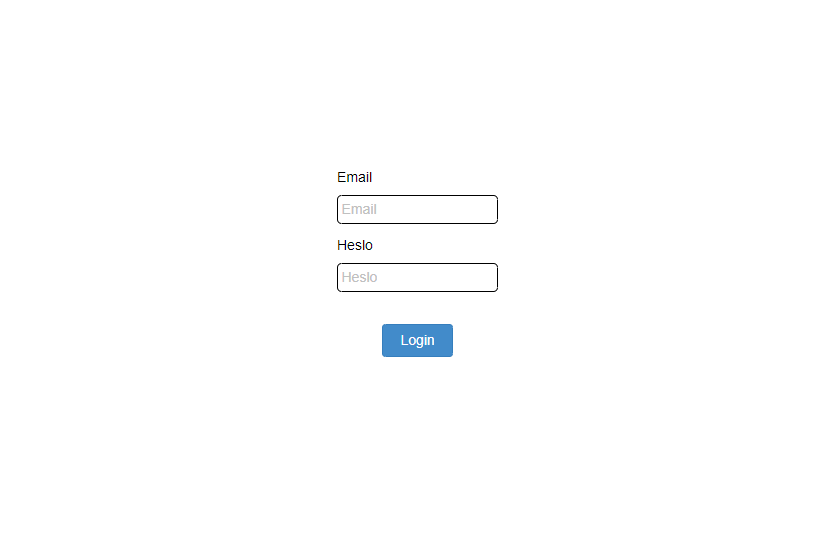
\includegraphics[width=\textwidth]{images/login}
        \caption {Přihlašování}
        \label {fig:login}
    \end{figure}

    \begin {figure}[H]\centering
        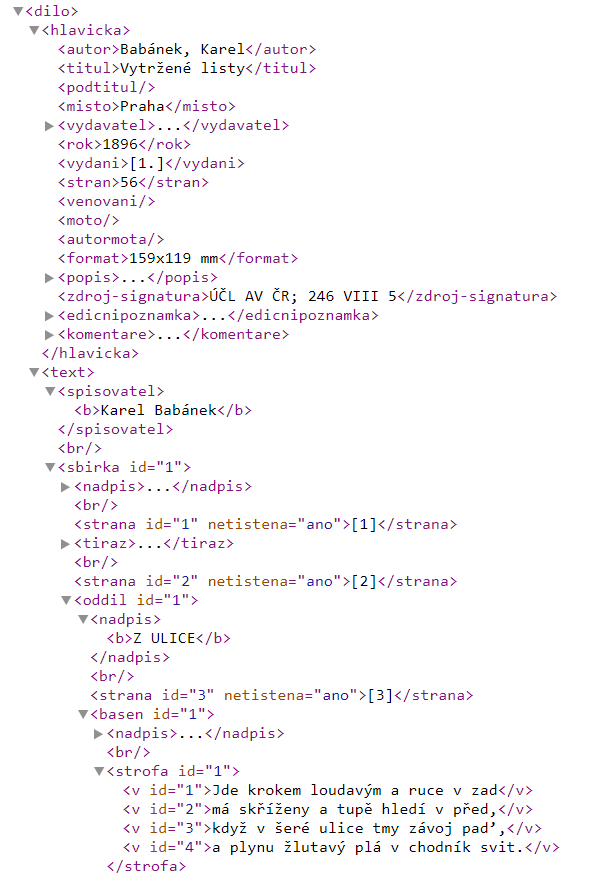
\includegraphics[width=\textwidth]{images/xml}
        \caption {Ukázka podoby díla}
        \label {fig:xml}
    \end{figure}   

    \begin {figure}[H]\centering
        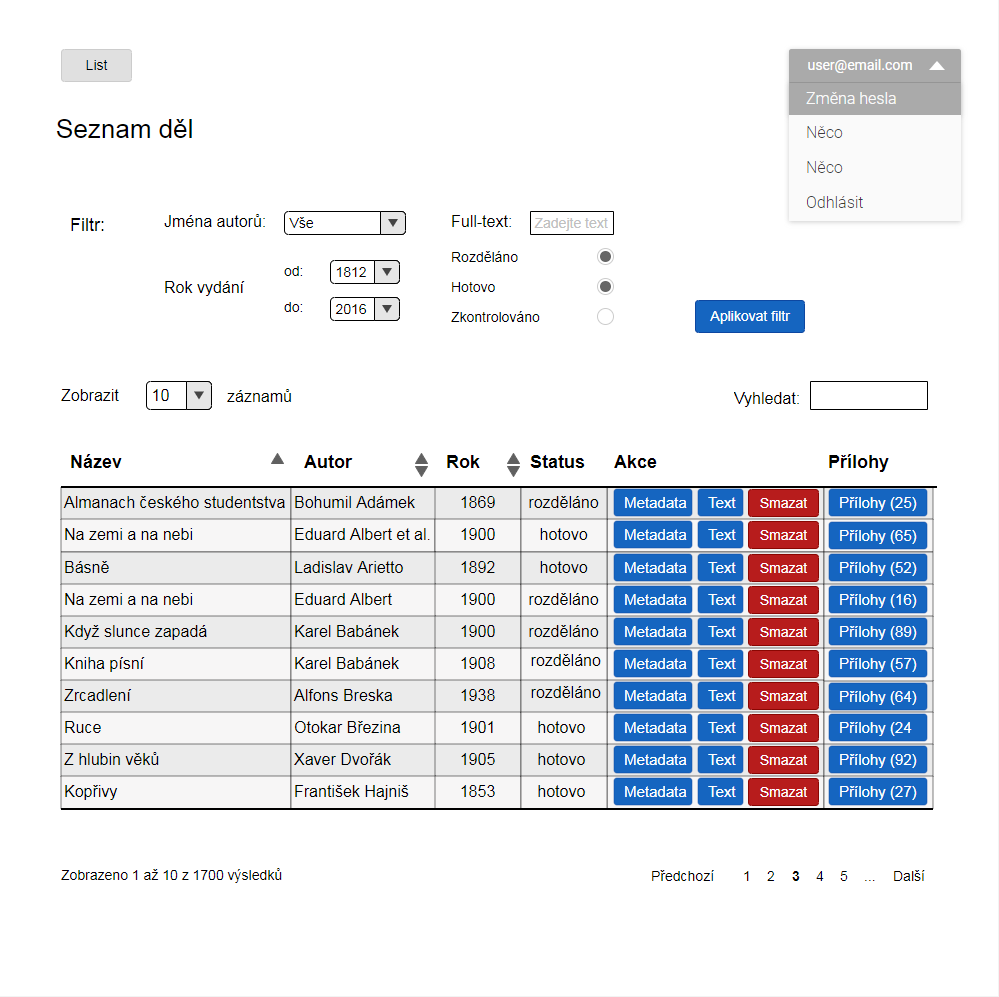
\includegraphics[width=0.991\textwidth]{images/main}
        \caption {Hlavní stránka}
        \label {fig:main}
    \end{figure}

    \begin {figure}[H]\centering
        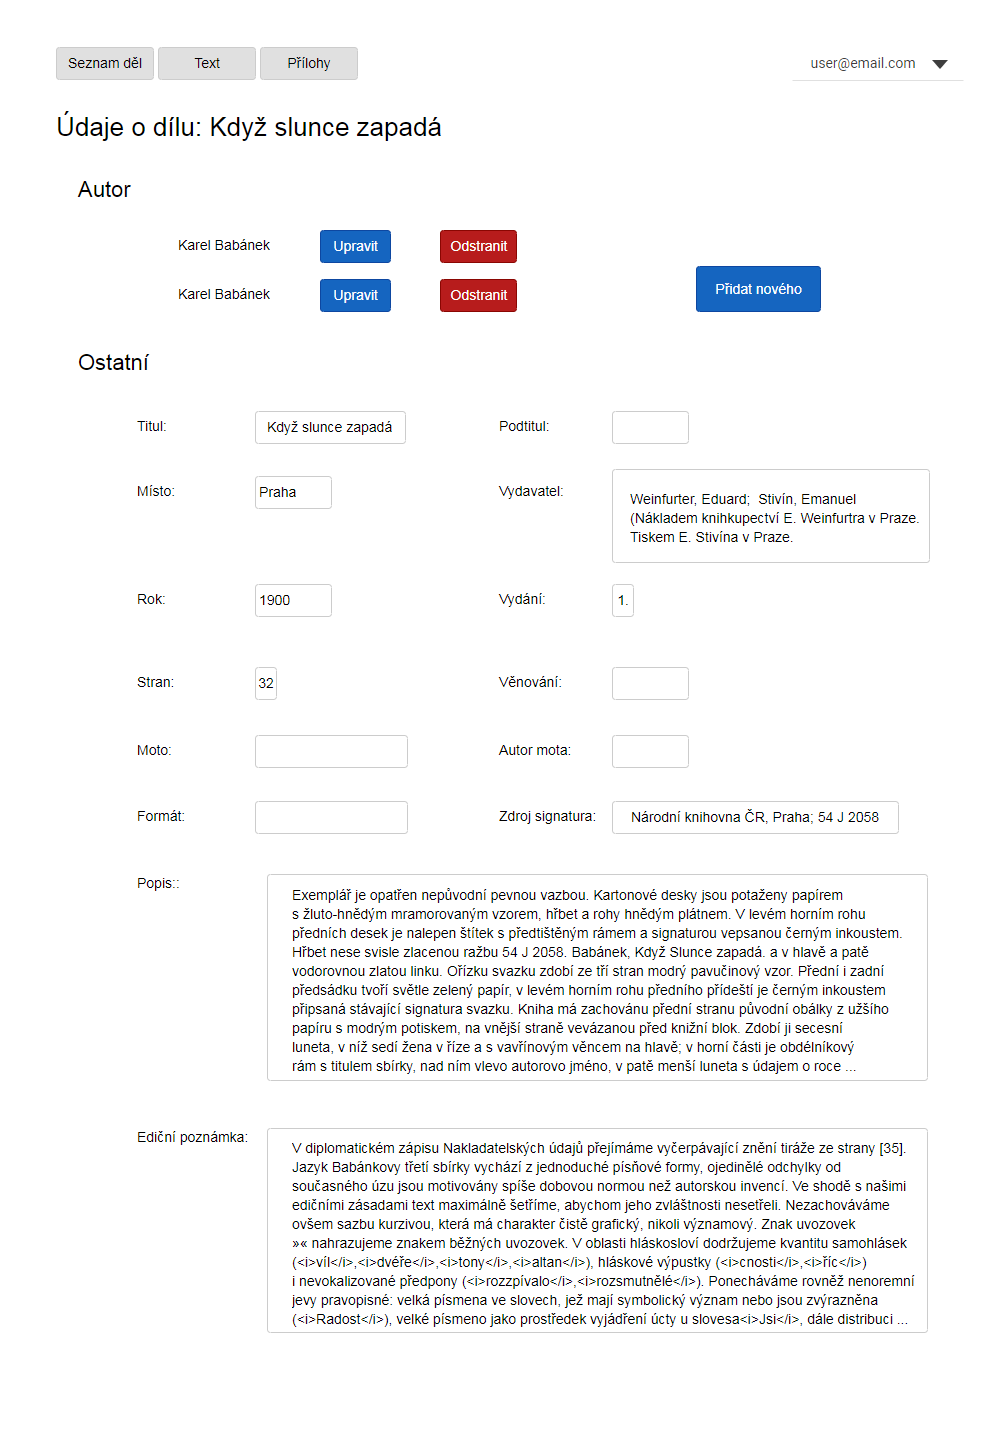
\includegraphics[width=\textwidth]{images/metadata}
        \caption {Metadata}
        \label {fig:metadata}
    \end{figure}
    
    \begin {figure}[H]\centering
        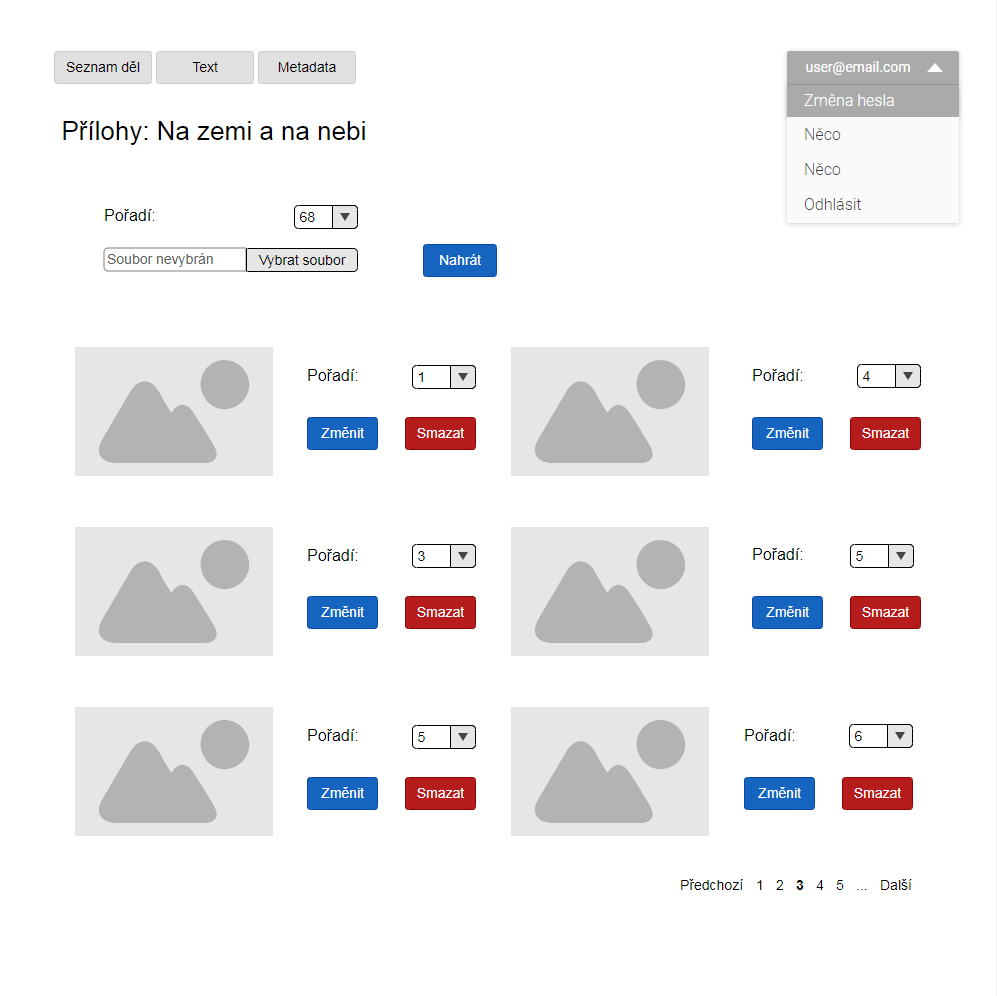
\includegraphics[width=\textwidth]{images/attachments}
        \caption {Přílohy}
        \label {fig:attachments}
    \end{figure}

    \begin {figure}[H]\centering
        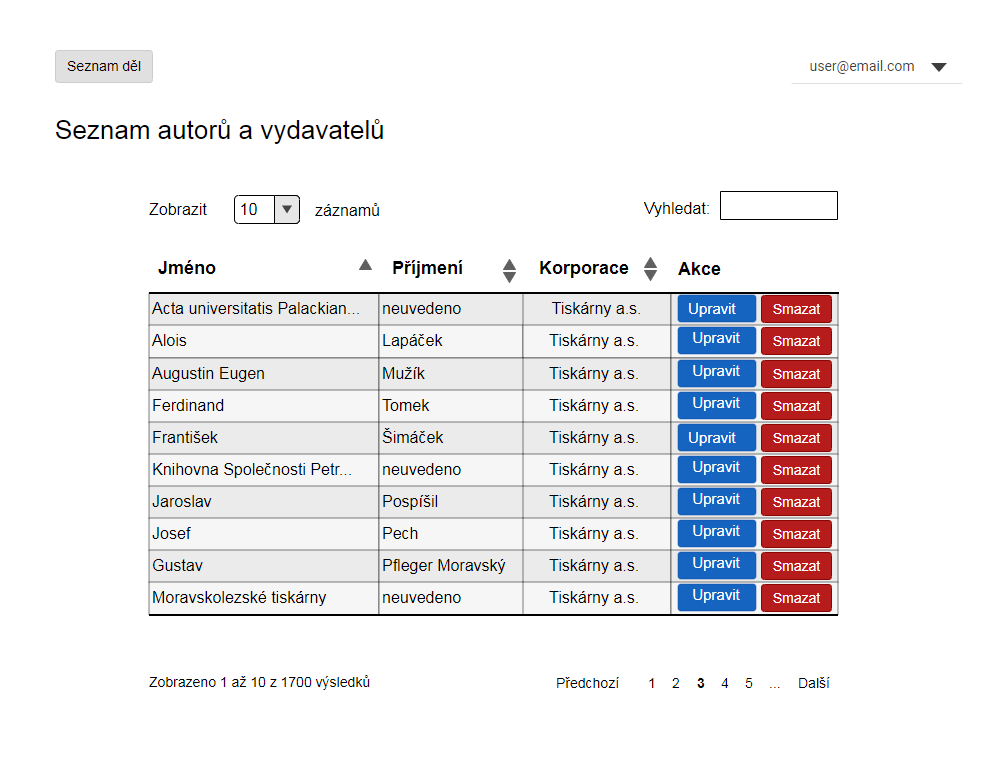
\includegraphics[width=\textwidth]{images/authPub}
        \caption {Seznam autorů a vydavatelů}
        \label {fig:authPub}
    \end{figure}
    
    \begin {figure}[H]\centering
        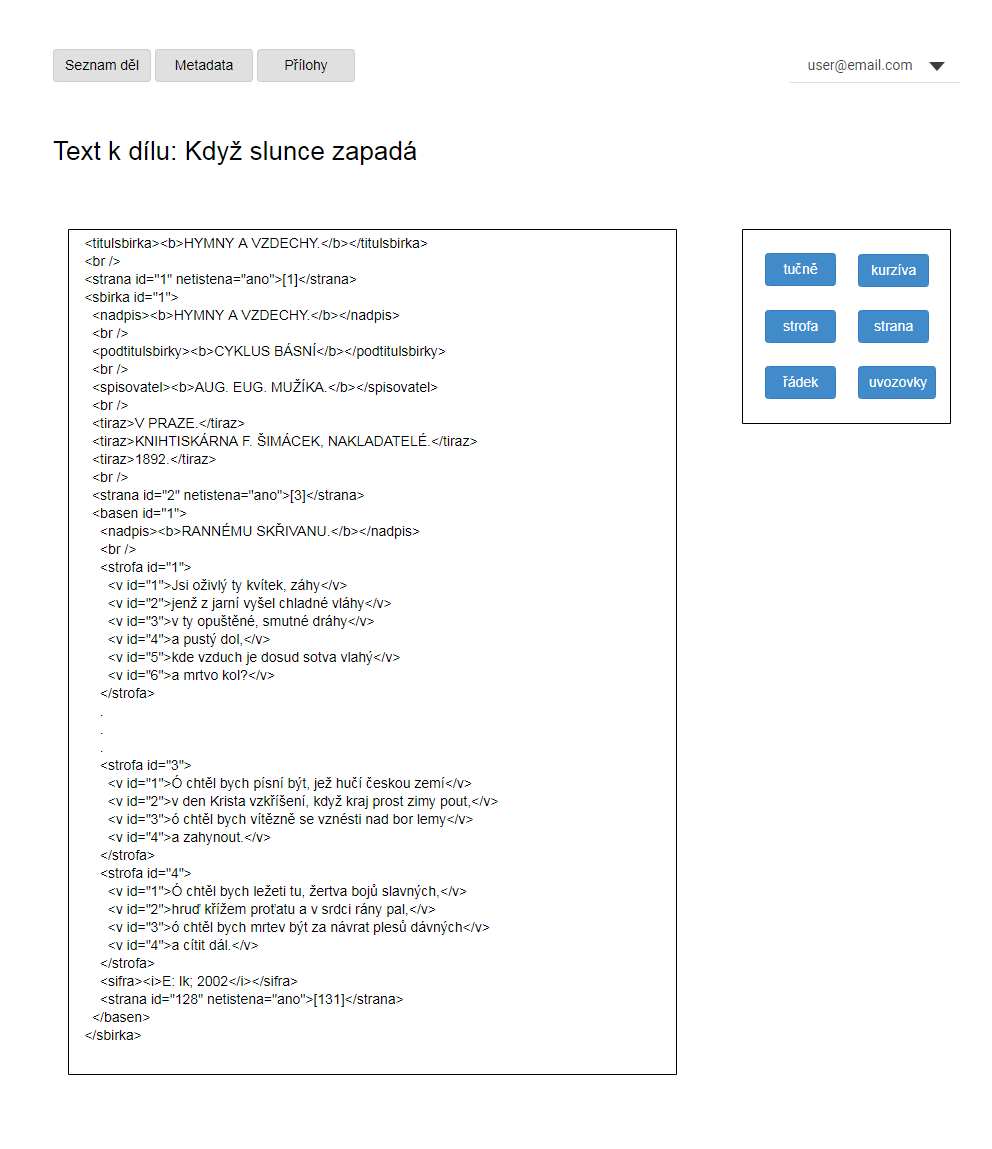
\includegraphics[width=\textwidth]{images/text}
        \caption {Text díla}
        \label {fig:text}
    \end{figure}
    
\chapter{Seznam použitých zkratek}
% \printglossaries
\begin{description}
	\item[GUI] Graphical user interface
	\item[XML] Extensible markup language
	\item[TEI] Text Encoding Initiative
	\item[HTML] HyperText Markup Language
	\item[JRE] Java Runtime Environment
	\item[UČL AV] Ústavu české literatury Akademie věd České republiky
	\item[ISS] Internet Information Services
	\item[DRM] Digital rights management
	\item[DIC] Dependency Injection Container
\end{description}


% % % % % % % % % % % % % % % % % % % % % % % % % % % % 
% % Tuto kapitolu z výsledné práce ODSTRAŇTE.
% % % % % % % % % % % % % % % % % % % % % % % % % % % % 
% 
% \chapter{Návod k~použití této šablony}
% 
% Tento dokument slouží jako základ pro napsání závěrečné práce na Fakultě informačních technologií ČVUT v~Praze.
% 
% \section{Výběr základu}
% 
% Vyberte si šablonu podle druhu práce (bakalářská, diplomová), jazyka (čeština, angličtina) a kódování (ASCII, \mbox{UTF-8}, \mbox{ISO-8859-2} neboli latin2 a nebo \mbox{Windows-1250}). 
% 
% V~české variantě naleznete šablony v~souborech pojmenovaných ve formátu práce\_kódování.tex. Typ může být:
% \begin{description}
% 	\item[BP] bakalářská práce,
% 	\item[DP] diplomová (magisterská) práce.
% \end{description}
% Kódování, ve kterém chcete psát, může být:
% \begin{description}
% 	\item[UTF-8] kódování Unicode,
% 	\item[ISO-8859-2] latin2,
% 	\item[Windows-1250] znaková sada 1250 Windows.
% \end{description}
% V~případě nejistoty ohledně kódování doporučujeme následující postup:
% \begin{enumerate}
% 	\item Otevřete šablony pro kódování UTF-8 v~editoru prostého textu, který chcete pro psaní práce použít -- pokud můžete texty s~diakritikou normálně přečíst, použijte tuto šablonu.
% 	\item V~opačném případě postupujte dále podle toho, jaký operační systém používáte:
% 	\begin{itemize}
% 		\item v~případě Windows použijte šablonu pro kódování \mbox{Windows-1250},
% 		\item jinak zkuste použít šablonu pro kódování \mbox{ISO-8859-2}.
% 	\end{itemize}
% \end{enumerate}
% 
% 
% V~anglické variantě jsou šablony pojmenované podle typu práce, možnosti jsou:
% \begin{description}
% 	\item[bachelors] bakalářská práce,
% 	\item[masters] diplomová (magisterská) práce.
% \end{description}
% 
% \section{Použití šablony}
% 
% Šablona je určena pro zpracování systémem \LaTeXe{}. Text je možné psát v~textovém editoru jako prostý text, lze však také využít specializovaný editor pro \LaTeX{}, např. Kile.
% 
% Pro získání tisknutelného výstupu z~takto vytvořeného souboru použijte příkaz \verb|pdflatex|, kterému předáte cestu k~souboru jako parametr. Vhodný editor pro \LaTeX{} toto udělá za Vás. \verb|pdfcslatex| ani \verb|cslatex| \emph{nebudou} s~těmito šablonami fungovat.
% 
% Více informací o~použití systému \LaTeX{} najdete např. v~\cite{wikilatex}.
% 
% \subsection{Typografie}
% 
% Při psaní dodržujte typografické konvence zvoleného jazyka. České \uv{uvozovky} zapisujte použitím příkazu \verb|\uv|, kterému v~parametru předáte text, jenž má být v~uvozovkách. Anglické otevírací uvozovky se v~\LaTeX{}u zadávají jako dva zpětné apostrofy, uzavírací uvozovky jako dva apostrofy. Často chybně uváděný symbol "{} (palce) nemá s~uvozovkami nic společného.
% 
% Dále je třeba zabránit zalomení řádky mezi některými slovy, v~češtině např. za jednopísmennými předložkami a spojkami (vyjma \uv{a}). To docílíte vložením pružné nezalomitelné mezery -- znakem \texttt{\textasciitilde}. V~tomto případě to není třeba dělat ručně, lze použít program \verb|vlna|.
% 
% Více o~typografii viz \cite{kobltypo}.
% 
% \subsection{Obrázky}
% 
% Pro umožnění vkládání obrázků je vhodné použít balíček \verb|graphicx|, samotné vložení se provede příkazem \verb|\includegraphics|. Takto je možné vkládat obrázky ve formátu PDF, PNG a JPEG jestliže používáte pdf\LaTeX{} nebo ve formátu EPS jestliže používáte \LaTeX{}. Doporučujeme preferovat vektorové obrázky před rastrovými (vyjma fotografií).
% 
% \subsubsection{Získání vhodného formátu}
% 
% Pro získání vektorových formátů PDF nebo EPS z~jiných lze použít některý z~vektorových grafických editorů. Pro převod rastrového obrázku na vektorový lze použít rasterizaci, kterou mnohé editory zvládají (např. Inkscape). Pro konverze lze použít též nástroje pro dávkové zpracování běžně dodávané s~\LaTeX{}em, např. \verb|epstopdf|.
% 
% \subsubsection{Plovoucí prostředí}
% 
% Příkazem \verb|\includegraphics| lze obrázky vkládat přímo, doporučujeme však použít plovoucí prostředí, konkrétně \verb|figure|. Například obrázek \ref{fig:float} byl vložen tímto způsobem. Vůbec přitom nevadí, když je obrázek umístěn jinde, než bylo původně zamýšleno -- je tomu tak hlavně kvůli dodržení typografických konvencí. Namísto vynucování konkrétní pozice obrázku doporučujeme používat odkazování z~textu (dvojice příkazů \verb|\label| a \verb|\ref|).
% 
% \begin{figure}\centering
% 	
\includegraphics[width=0.5\textwidth, angle=30]{cvut-logo-bw}
% 	\caption[Příklad obrázku]{Ukázkový obrázek v~plovoucím prostředí}\label{fig:float}
% \end{figure}
% 
% \subsubsection{Verze obrázků}
% 
% % Gnuplot BW i barevně
% Může se hodit mít více verzí stejného obrázku, např. pro barevný či černobílý tisk a nebo pro prezentaci. S~pomocí některých nástrojů na generování grafiky je to snadné.
% 
% Máte-li například graf vytvořený v programu Gnuplot, můžete jeho černobílou variantu (viz obr. \ref{fig:gnuplot-bw}) vytvořit parametrem \verb|monochrome dashed| příkazu \verb|set term|. Barevnou variantu (viz obr. \ref{fig:gnuplot-col}) vhodnou na prezentace lze vytvořit parametrem \verb|colour solid|.
% 
% \begin{figure}\centering
% 	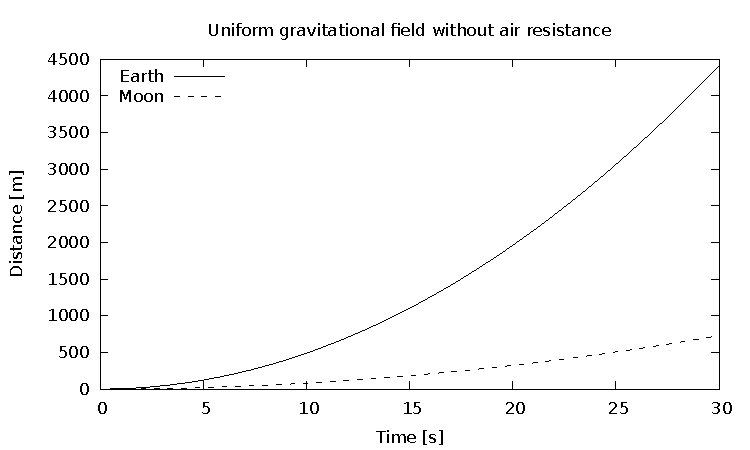
\includegraphics{gnuplot-bw}
% 	\caption{Černobílá varianta obrázku generovaného programem Gnuplot}\label{fig:gnuplot-bw}
% \end{figure}
% 
% \begin{figure}\centering
% 	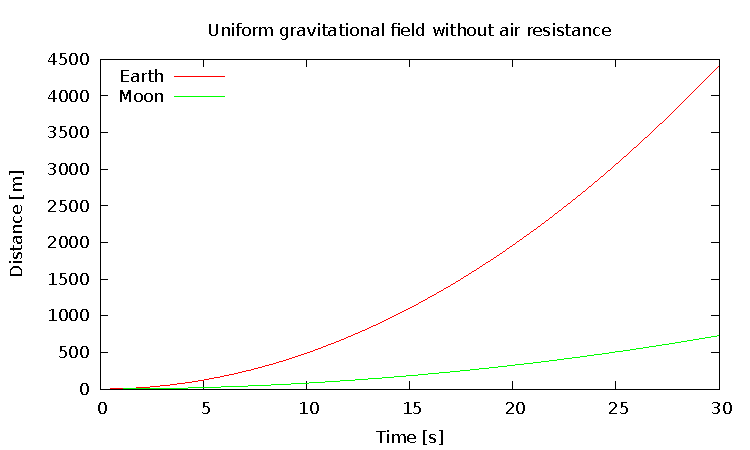
\includegraphics{gnuplot-col}
% 	\caption{Barevná varianta obrázku generovaného programem Gnuplot}\label{fig:gnuplot-col}
% \end{figure}
% 
% 
% \subsection{Tabulky}
% 
% Tabulky lze zadávat různě, např. v~prostředí \verb|tabular|, avšak pro jejich vkládání platí to samé, co pro obrázky -- použijte plovoucí prostředí, v~tomto případě \verb|table|. Například tabulka \ref{tab:matematika} byla vložena tímto způsobem.
% 
% \begin{table}\centering
% 	\caption[Příklad tabulky]{Zadávání matematiky}\label{tab:matematika}
% 	\begin{tabular}{|l|l|c|c|}\hline
% 		Typ		& Prostředí		& \LaTeX{}ovská zkratka	& \TeX{}ovská zkratka	\tabularnewline \hline \hline
% 		Text		& \verb|math|		& \verb|\(...\)|	& \verb|$...$|		\tabularnewline \hline
% 		Displayed	& \verb|displaymath|	& \verb|\[...\]|	& \verb|$$...$$|	\tabularnewline \hline
% 	\end{tabular}
% \end{table}
% 
% % % % % % % % % % % % % % % % % % % % % % % % % % % % 

\chapter{Obsah přiloženého CD}

%upravte podle skutecnosti

\begin{figure}
	\dirtree{%
		.1 readme.txt\DTcomment{stručný popis obsahu CD}.
		.1 exe\DTcomment{adresář se spustitelnou formou implementace}.
		.1 src.
		.2 impl\DTcomment{zdrojové kódy implementace}.
		.2 thesis\DTcomment{zdrojová forma práce ve formátu \LaTeX{}}.
		.1 text\DTcomment{text práce}.
		.2 thesis.pdf\DTcomment{text práce ve formátu PDF}.
		.2 thesis.ps\DTcomment{text práce ve formátu PS}.
	}
\end{figure}

\end{document}


